\chapter{TCP/IPの概論}

TCP/IPはいまいちわかりにくいですよね。

インターネットを経由しての通信は、TCP/IPで行われているのは知っているでしょう。でも、アプリケーションから見たとき、TCPとかIPとかがどんな役割をしているから、離れたサーバとクライアントが通信できるのか。また、LANとインターネットとはどんな風に繋がっているのか。そんな部分がよくわからない。

まずは、TCP/IPというもののイメージを掴んでみることにしましょう。

この章では、通信を行う両社を、慣例に従ってAliceとBobという名前で表記します。

\section{鳥類キャリアによるIP伝送}

伝書鳩でインターネット通信ができる。そのための規格があることをご存知だろうか。

インターネットにおける規格を提案するRFC\footnote{Request for Comment}の1149番で、鳥類キャリアによるIP伝送(IPoAC IP over Avian Carrier)という規格が提案されている。\footnote{https://tools.ietf.org/html/rfc1149}

IPoACについて簡単に説明すれば、紙に通信したいデータを書いて、伝書鳩\footnote{規格ではavian carrierであり、伝書『鳩』と明記はされていない}にくくりつけて飛ばす、そうやってインターネットの通信を行う手順の提案である。
このように、IPoACは、鳩に持たせるための紙に書いたデータを作成する規約、鳩の挙動などについて言及し、伝書鳩をインターネットの通信に使用できるようにした規格の提案として提出されたものだ。

種を明かせば、IPoACは1990年4月1日に発行された提案であり、ジョークRFCと呼ばれるもののひとつである。RFCでは、毎年4月1日非は、このようなジョークRFCを発行する習慣がある。

IPoACはジョークRFCではあったが、実証実験が行われている。その実証実験では、鳩が宛先に辿り着かなかったことによって生ずるデータの損失が多く、鳩なので伝送遅延も大きい。つまり、通信のやり直しや通信そのものにかかる時間が大きいという、ある意味当然の結論が出た。
だが、IPoACは、これらの問題を許容すれば、伝書鳩でインターネットの通信を行うことが可能であることも、その実証実験でしめした。



\section*{}
\begin{itembox}[l]{いもうとコラム 惑星間インターネット}
RFC1149はいわゆるジョークRFCでしたが、、インターネット通信において、送ったデータのロストや応答時間(レイテンシ)が大きくなる環境があります。
それは、宇宙です。さよならジュピターでも、カイパーベルト領域ま行った探査船のコンピュータであるナヴァホと、月に設置されたコンピュータのティム・ラビットがレイテンシを越えて会話するシーンがありました。

このような環境のインターネット通信は、惑星間インターネット(Interplanetary Internet)として研究開発が行われています。
\end{itembox}


\section{伝書鳩でインターネットの通信をするための仕組み}
鳩は遅い。そして、送り出した鳩が、目的とする通信相手にたどり着くわけでもない。また、順番通りに届くわけでもない。だが、鳩を伝送媒体に用いて、でインターネットで行われている通信が成立する。

そのような条件で通信ができるようにするには、どうすればよいのだろうか。それは、伝送遅延を許容し、鳩は確率的にしか相手のところにたどり着かず、送り出した順番と到着した順番が一致しないことを前提に通信の仕組みを作る。つまり、鳩に完璧さを求めず、それをサポートする仕組みをつくれがよい。

伝書鳩の役割とは、通信を行う双方の間で、情報を物理的な空間を越えて運ぶことである。
鳩なので、途中で餌になる虫を見つけたり、発情期で交尾相手を見つけたり、鷹に追いかけられて逃げたりするかもしれない。これらの可能性は、IPoACでも検討されている。
鳩は、通信の焚いての所に到着する時間がわからない。それどころか、相手のところに到着しないこともある。送り出した順番に鳩が到着することもないだろう。

まず、鳩なのだから、必ずしも通信の相手側に到着するわけではない。これを前提条件として、伝書鳩で通信をするための仕組みを考えて聞くことにしよう。


\subsection{鳩を使って確実な通信をする方法}

現在のインターネットは、確実な通信を行っている。だが、IPoACを使ってインターネットの通信を行うのうなら、データを運ぶ手段が鳩であるという前提で、確実な通信をおこなう手段をかなが得なければならない。
それは、相手にデータが届いたことがわかるまで、同じデータを送り直し続ける、ということである。この過程をくりかえしていけば、確率的にいつか通信が成功するだろう。


最初に、AliceとBobで、鳩が行き来できる状況なのかを確認する。その確認が取れないと、いくら鳩を飛ばしても通信が成立しない可能性があるということだ。

次に、鳩が届けたデータを受け取った側は、Aliceに向けて飛ぶ鳩を使って、データを受け取ったという返事をすることにする。
このとき、データを運ぶ手段は鳩しかない。電話など、鳩以外の手段で通信を届けることはできない。

三つ目、データを送信した側は、一定時間待って、データを受け取ったことを知らせる鳩が通信お相手から来なければ、送り出した鳩が到着しなかったとみなして、もう一度鳩を送り出す。
これは、相手がデータを受け取ったことが確認できるまで3は、そのデータは届いていないと見なして再送する、ということである。

最後に、送信するデータには、送信した順番を再現するための通し番号を書いておく。受信したというメッセージには、その番号も書き添え、何番目のデータを受け取ったかがわかるようにする。

この手順は、TCP/IPで、確実な通信を行うため仕組みを、ごく簡単にしたものである。


\subsection{鳩の遣り取りができるかの確認}

最初に、Aliceから、鳩が相手にたどり着ける状況にあるのかを確認する。その方法は、通信を開始したい、という内容のデータを持った鳩を、Bobにとばす。
そのはとを受け取ったBobは、鳩が届いた、こちらも通信できる、というデータを持たせた鳩を、Aliceにとばす。Aliceにその鳩が到着したら、Aliceは、鳩を飛ばしても大丈夫だと知ることができる。
次にAliceは、鳩が到着した、というデータを持たせた鳩を、Bobに送る。これによって、Bobは、Aliceと鳩の遣り取りができる状況なのを知ることができる。

このように、AliceとBobが鳩を送りあって状況を確認することは、TCPの3way-Handshakeという動作似相当する。


\subsubsection{AliceとBobの協調}
次に、IPoACで、AliceとBobはどのくらい協調して通信を行うのだろうか。
前提として、この両者は、鳩以外の情報伝達手段を持っていないことを再度確認しておきたい。変な言い方ではあるが、我々はインターネットで通信を行う際に、インターネットしか情報伝達手段を持っていない。

Aliceは、データを送る必要がある場合は、Bobへの事前連絡なしに鳩を放つ。
IPoACでは鳩より早い情報伝達手段がない前提である。そのため、事前連絡のしようもない。
そのため、Bobは、いつ鳩がきてもいいように受け入れる準備をしている。だが、鳩がこない限りは何もしない。大切なことなのでもう一度書くと、鳩より速い通信手段はないのだ。なので、Aliceに事前の連絡を取ることはできないない。

Bobから送られる、到着したという情報についても同様である。Bobは、Aliceへの事前連絡なしに、到着したという返事を持たせた鳩を放つ。
Aliceは、到着した、という連絡を持った鳩がいつ来てもいいように準備している。だが、鳩が来ずにに時間切れになったら、こんどはAliceがBobへの事前連絡なしに、先ほど送り出した鳩と同じデータを持った鳩を送り出す。

これは、TCP/IPにおける、TCPがデータを確実に届ける手順二層等する。

\subsubsection{到着した鳩の順番が違っていた場合}
到着した鳩が持っていたメッセージの順番が違っていた場合は、どのようにすれば良いだろうか。たとえば、1番データを持った鳩が来たが、次に来たのは3番のデータを持った鳩であった場合である。2番のデータが来てないことはどう連絡すればいいだろうか。

Bobは、1番のデータが届いた、という応答を、鳩を使ってAliceに送る。だが、2番のデータに関しては何もしない。そもそも、2番のデータが存在するかわからないのだ。来ないという連絡のしようもない

Aliceは、2番のデータが「受信できた」というメッセージが来なかったことで、2番以降のデータを送り直す。2番のデータだけ送り直すのではない。一見無駄が多いようだが、こうすることで、どの鳩の到着の連絡があったかの管理をせずに済むというメリットがある。


\subsection{鳩の到着の連絡を省略する通信}
ここまで説明した方法は、データを受け取った、というメッセージのやりとりが成立するまで、り鳩が再び放たれ続ける。正直なところ、これは面倒だし、鳩の到着と、それを知らせる鳩の送出のコスとは、、Alice、Bobのどちらにとっても高い。そのため、受信した、という確認を省略する通信というものがある。

たとえば、一匹の鳩の脚にくくれる程度の問い合わせと、おなじく一匹の鳩の脚にくくれる答えで終了する通信があるとする。このとき、到着した、という連絡にかける手間は、行われる通信のデータ量に対して、あまりにも大きい。
そのため、確実性がなくてもかまわない場合は、到着したという連絡を省略することで、通信のコストダウンを計ることができる。

このような、受信の確認を省略する通信は、TCP/IPにおけるUDPに沿うとする。

\subsection{鳩が飛ぶ先の表し方}
IPoACで通信を行うとき、鳩はどこに向けて飛ばすのか。伝書鳩は、ある宛先にむけて飛ぶように訓練される。つまり、宛先ことに、そこに向けて飛ぶ鳩を用意して、決定した宛先によって鳩を選択する。

鳩を飛ばす人間は、宛先をどのように管理するのだろうか。それには、住所表示を使うことにしよう。そうすることで、鳩を管理する人間が、どこに飛ぶ鳩を使うのか管理しやすくなる。

\subsection{二つの住所表示}

京都市は、住所の表し方が二つある。何区何町何丁目何番地、という表し方は、通常の住所表示として使われる。
だが、古い表現として、街路が碁盤の目になっている京都では、場所のブロックがどの通りに面しているかを、東西方向、南北方向の通りの交差点から、東西南北どちらに進めばいいかで表現するやりかたがある。

たとえば、京都市役所は、現在使用されている住所表記では京都市中京区押小路河原町西入榎木町450-2であるが、古い表記では京都市中京区寺町通り御池上ル本能寺前となる。
だが、京都市役所を宛先とする郵便を出すときは、このどちらで記載しても届く。\footnote{京都では、古い住所表記に使われる通りの名前を、「まるたけえびすに、おしおいけ、あねさんろっかく」というような歌にして覚えていた。この歌はいくつかあるので、興味があれば調べてみてほしい。}

京都の住所表記に着いて説明したのは、ひとつの場所を表す住居放棄に、複数の表現方法がある場所としてだ。古い表記は比較的おおざっぱ、新しい表記は細かい。だが、実際の地図上の場所は同じである。
新しい表記は、より細かく場所を特定することができる。つまり、本能寺前に市役所以外の建物があったとしても、番地の番号まで使えば、市役所とは別の住所としてで表すことができるだろう。

だが、そんな違いがあったとして、メッセージを作る人間は、京都市役所という場所を宛先として指定する。住所の表記の違いは、京都市中京区寺町通り御池上ル本能寺前「」に向けて飛ぶ鳩を使うのか、京都市中京区押小路河原町西入榎木町450-2「」にむけて飛ぶ鳩を使うのか、という使い分けを行うことに相当する。

この二種類の表記は、後に説明するIPv4とIPv6に対応する。



\subsection{鳩と人間の役割分担}
次に、IPoACを使った通信での、鳩と人間の役割分担について考えてみよう。そのために、鳩と人間がIPoACにおいてどのように振る舞うかを再確認したい。





\subsection{IPoACとインターネットプロトコルモデル}
では、実際のインターネットにおいて、鳩はどこにいるのだろうか。正確に言えば、鳩に相当するのはどの部分なのだろうか。
それを考えるために、IPoACを、実際のインターネットに相当するモデルに当てはめてみよう。
ここまで説明した内容で、メッセージを作ってからはとを送り出すまでの手順を分けて書いてみると、表\ref{hatostack}のように現せる。

\begin{table}[hbtp] 			
\begin{center} \label{hatostack}
	\begin{tabular}{l}  \toprule
		役割 \\ \midrule
		メッセージをデータとしてを作る \\
		データの送受信の管理 \\
		鳩を飛ばし受け入れる \\
		鳩がデータを運ぶ \\ \bottomrule
	\end{tabular}
\end{center} \caption{人と鳩の役割分担}
\end{table}

これをインターネットの用語に置き換えてみよう。説明はこの先で行うので、今はインターネットでの用語が何になるかだけ見てもらうのでかまわない。

\begin{table}[hbtp] 
\begin{center} \label{hatostack2}
	\begin{tabular}{ll} \toprule
		役割 & インターネットでの名称 \\ \midrule
		メッセージをデータとしてを作る & アプリケーション層 \\
		データの送受信の管理 & トランスポート層 \\
		鳩を飛ばし受け入れる & インターネットプロトコル層 \\
		鳩がデータを運ぶ & ネットワークコミュニケーション層 \\ \bottomrule
	\end{tabular}
\end{center} \caption{インターネットの用語との対応関係}
\end{table} 

表\ref{hatostack2}のように、メッセージを作るものをアプリケーション層、データの送受信を管理するトランスポート層、鳩を送り出し、受け入れるのがインターネットプロトコル層、鳩そのものが、ネットワークアクセス層とよばれる、それぞれの層(レイヤー)に相当する。

この四つの機能が菱餅のように重なり合っているイメージでとらえられることから、いわyるるTCP/IPのことを、インターネットプロトコルモデルと呼ぶ。

\subsection{プロトコル}
プロトコル(Protocol)という言葉は、何を意味するのだろうか。辞書では、外交手順、儀礼、議定書、という意味の単語である。ネットワークにおけるプロトコルとは、ネットワーク機器が相互に通信を行うための規約、規格のことである。TCP/IPという名前は、Transmission Control Protocol/Internet Protocolsというように、二つのプロトコルという言葉が含まれている。

IPは、複数の異なるネットワークの間で通信を行うための規約である。また、TCPは、IPのサービスをデータの伝送のために利用して、確実にデータを届けるための規約である。

TCP/IPは、TCPとIPだけでなく、UDPや各種のアプリケーション層のプロトコルというように、複数のプロトコルが集まった規格である。このような、各種のプロトコルが集まって成り立っている規約を、プロトコルスイートと呼ぶ。
インターネットプロトコルスイートは、インターネットの通信のための規約の集合体である。

\section*{}
\begin{itembox}[l]{いもうとコラム IPoACは何を定義しているのか}
実際のところ、IPoACは何を定義しているのでしょうか。それをインターネットプロトコルスイートの言葉を使うと、ネットワークコミュニケーション層である鳩に、どのようにインターネットプロトコル層でのデータを載せ、取り扱うのか、という部分になります。

これは名前からもわかることで、IPデータグラムを鳩に乗せて運ぶから、IP over Avian Carriersとなるのです。

\end{itembox}


\section{インターネットプロトコルスイートとTCP/IP}

\begin{table}[hbtp] 
\begin{center} \label{internetprotocolsuite}
	\begin{tabular}{l}  \toprule 
		レイヤ名 \\ \midrule
		アプリケーション層 \\
		トランスポート層 \\
		インターネットプロトコル層 \\
		ネットワークアクセス層 \\ \bottomrule
	\end{tabular} \caption{インターネットプロトコルスイート}
\end{center}
\end{table}

インターネットの通信方法であるTCP/IPは、このように、役割分担した機能を組み合わせることでできている。そのため、このモデルをインターネットプロトコルスイート、と呼んでいる。また、その機能の一つ一つに層(レイヤ)という言葉がつくのは、表\ref{internetprotocolsuite}のように、上下に層となって重なっているように表されるためだ。


では、ここまで何となく使ってきたTCP/IPという用語は何であろうか。TCPはトランスポート層のプロトコルの一つ、IPはインターネットプロトコル層のプロトコルの名称である。一見すると、表\ref{internetprotocolsuite}の、トランスポート層とインターネットプロトコル層のプロトコルの名前をつなげただけに見える。
だが、TCP/IPと言うときは、インターネットプロトコルスイートそのものを現す名前となる。

\subsection{レイヤの上下関係とサービス}

\begin{wrapfigure}[17]{r}{6cm}
	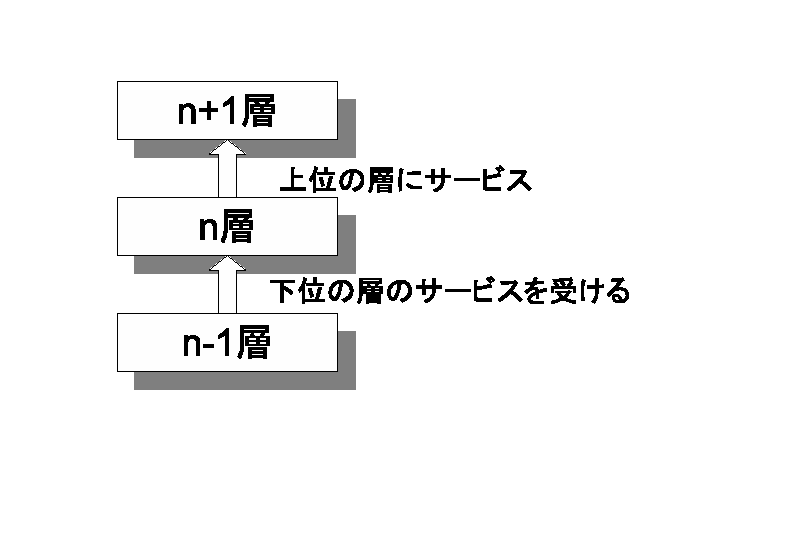
\includegraphics[width=6cm, clip]{draw/service.eps}
	\caption{レイヤの上下関係}
	\label{fig:service}
\end{wrapfigure}

インターネットプロトコルスイートの各層は、自分より下の層が自分にサービスすることを前提に、自分より上の層に対してサービスを行う。

もういちどIPoACで説明すれば、インターネットプロトコル層は、ネットワークコミュニケーション層である、鳩がデータを運ぶのを利用してデータを送り出し、受け入れる。そして、受け入れたデータをトランスポート層にわたし、トランスポート層から送り出すべきデータを受け取る。インターネットプロトコル層は、鳩がデータを運んでくれれば、途中でどんな飛び方をするか、そして、鳩が到着するかどうかについては、全く関知しない。
そして、トランスポート層には求められるサービスを提供するだけで、トランスポート層が何をしているかは全く関知しない。

このことを、あるレイヤーが下から数えて$n$番目にあるとき、$n$層のサービスは、$n-1$層からサービスを受け、$n+1$層にサービスする、といううように言い表す。

\subsection{レイヤ間の依存関係とプロトコルスタック}

層の間の依存関係はどうであろうか。実は、それぞれの層は、お互いに全く依存しあわない。
ネトワークコミュニケーション層として鳩を使うかわりに、糸電話を使っても、瓶詰めの手紙を海に流しても、はじめてのお使いをする姪っ子に持たせても、通信は成立する。このことを表す言葉として、Two can and tin. というフレーズがある。意訳すれば「糸電話でもいいよ」となる。

これは、あるレイヤは、直接に接していないレイヤのことは全く気にする必要がないということでもある。トランスポート層は、情報を運ぶ何かが鳩なのか糸電話なのか、それとも姪っ子なのかを考える必要がない。

また、本書ではインターネットプロトコル層について、バージョン4のIPv4とバージョン6のIPv6の両方について、説明を行う。
インターネットプロトコル層が、IPv4とIPv6のどちらでも、トランスポート層、ネットワークアクセス層は、プロトコルの変更なく通信を行うことができる。\footnote{実装の観点で見れば、インタフェイスの違いなどから、全く変更が必要ないわけではない。}

トランスポート層の置き換えの例もある。インターネットの通信でWAN高速化を行う機器がある。これは、対向する機器の間でトランスポート層で、TCPやUDPなどの従来のプロトコルと違うものに置き換えて、通信時間の短縮を計る。このような通信が成立するのは、インターネット層が、トランスポート層が何をやっているかを関知しないためである。

ここまで説明したように、TCP/IPは異なった役割をもつプロトコルが、お互いにサービスを提供したりされたりして成り立っている。図にすると、各層のプロトコルを上下に重ねたように表される。このように、役割を分けたプロトコルが上下に重なる形で全体像が作られるプロトコルスイートを、プロトコルスタックと呼ぶ。


\section{エンドツーエンド原則}
TCP/IPには、二つの意味を持つエンドツーエンド原則というルールがある。ひとつは、通信の処理は、通信の当事者である両端でのみ行い、途中経路は関与しないという設計思想である。そして、もうひとつは、通信の当事者は対等であるべきという思想的なものとなる。

\subsection{処理は両端(エンド)でのみ行なう}

アプリケーション層やトランスポート層による制御は、通信の端点(エンド)側だけで行い、途中の経路は通信の導管に徹する、という宇設計思想である。
TCP/IPの用語では、途中の経路は、ネットワークコミュニケーション層と、インターネットプロトコル層までが関与する。そして、トランスポート層やアプリケーション層での通中に介在しない。そうすることで、通信のエンドとなる機器にのみ、トランスポート層やアプリケーション層を実装すればよいことになる。

TCP/IPは、途中経路の実装を簡単にして、経路の敷設を行いやすくする設計思想であった。トランスポート層以上の動作には、かなりのリCPUのソースを必要とした。そのため、重い処理をするノードを減らしたかったという、歴史的な事情もある。

設計士粗糖としての根戸ツーエンド原則は、コンピューターリソースが潤沢となった現在では、厳密に守られることはなくなった。プロキシなど、トランスポート層以上の動作をする者が、通信の途中に介在することもあるためである。

\subsection{通信の両端は常に対等である}

もう一つは、インターネットに接続されたすべてのエンドは、対等な立場で通信が可能であるべきという原則である。対等な立場というのは、インターネットに接続されたすべてのホストは、自分を含むすべてのホストに対して送信を行うことができ、逆に、すべてのホストからの通信を受信できるべき、ということである。

もっとも、現在のインターネットはこのエンドツーエンド原則の理念は失われている。犯罪対策のブロッキングは、経路で他のホストへの通信を制限してしまう措置である。
だが、エンドツーエンド原則が提唱された当時は、インターネットに接続していた組織がすべて顔見知りであった、いわゆる性善説が成り立っていた時代であることを記載しておかなければ不公平になるであろう。

\section*{}
\begin{itembox}[l]{いもうとコラム 実際のエンドツーエンド}
エンドツーエンドは、今ではあまり現実的でない考えであるという見方もあります。たとえば、プロキシやファイアウオールは、インターネットプロトコル層よりも上のレイヤーで通信を処理し、中継したり、通信を遮断します。

それでも、両端から見てインターネット層の通信で結ばれているように見えれば、通信は成立するということでもあります。それが、インターネットプロトコルの通信を、アプリケーション層のデータとして運ぶ「トンネル」の考え方につながっています。


\end{itembox}


\section{レイヤごとの役目とデータの名前}
では、各層の役目を、もう少しだけ、インターネットの用語を使って説明し直そう。また、隠れいやーで取り扱うデータには、それぞれ名前がある。

\subsection{ネットワークコミュニケーション層}
同じネットワークの中で、ネットワークに接続されたインタフェイスを区別し、通信するための層である。同じネットワークとは、二つ以上の機器が、共有する伝送媒体によって直接に接続されたものである。
ケーブルや信号などの電気的な規格と、それを利用してでどのような情報を送るか、それらをまとめが概念がネットワークコミュニケーション層である。

概念と書いたのは、ネットワークアクセス層そのものはTCP/IPでは定義されていないためだ。本書では後の章で、説明のためにPPPやイーサネットを取り上げているが、これらはインターネットプロトコルスイートの中でなく、別の規格をネットワークコミュニケーション層として利用しているものである。

ネットワークコミュニケーション層のデータを、フレームと呼ぶ。

\subsection{インターネットプロトコル層}
インターネットプロトコル層は、ネットワークコミュニケーション層でいうネットワークが複数あった場合に、そのネットワークとネットワークの間での通信を担当する。ただし、インターネットプロトコル層は、ネットワーク間の通信手段を提供するのが役目であり、確実に通信が成立しているかは保証しない。

IPアドレスは、インターネットプロトコル層でネットワークとそこに接続されたホストを特定するための識別手段であり、インターネットにおける文字通りの住所である。

インターネットプロトコル層では、これまで使われてきたIPバージョン4と、より多くのIPアドレスが使える、新しい規格のIPバージョン6という、二つのバージョンのインターネットプロトコル層の規格が、2018年現在は併用されている。IPv4とIPv6は同時に使用することが可能であり、同時に使用されていることを、IPv4をインターネットプロトコル層とするスタックと、IPv6をインターネットプロトコル層とするスタックの二つガルという意味で、デュアルスタックという。

インターネットプロトコル層のデータを、IPデータグラムと呼ぶ。また、IPパケット、という呼ぶこともある。これは、送り出され卯だけのデータを、電信(テレグラム)や小包(パケット)に見立てたものである。

\subsection{トランスポート層}
トランスポート層には大きく二つの役割がある。一つは、ポート番号とよばれる、通信を行うアプリケーションを特定するための番号を提供して、一つのIPアドレスを用いて複数のアプリケーションが同時に通信できるようにする、多重化である。
多重化は、TCPとUDPに共通する機能である。

もう一つは、TCPの昨日で、エンドツーエンドでの確実な通信を担保することである。確実な通信が成立している条件は、通信相手がデータを受信したことを確認した状態であるとする。また、データの到着順、つまり通信内容の送信順を確認して、データのっじゅしん側でその順番を再現する、つまり、通信の順番も担保している。

トランスポート層のデータは、プロトコルごとに異なる名前で呼ばれる。TCPのデータをセグメント、UDPのデータを、UDPデータグラムと呼ぶ。後ほど説明するが、UDPのデータは、IPデータグラムとほぼ同じ性質を持つため、区別してUDPデータグラムと呼ばれる。

\subsubsection{コネクションとコネクションレス}
TCPのように、確実な通信を行うプロトコルは、その動作から通信のエンド同士が直接接続されているかのような状態をエミュレートしていると考えることができる。そのため、コネクション型、もしくはコネクション指向の通信と呼ぶ。古い資料では、電話交換網でエンドとエンドの間が電話線で結ばれている状態に見立てて、仮装交換回路(バーチャルサーキット)と呼んでいるものがある。

一方のUDPは、確実な通信を行うために必要な、「受信した」追う乙の送出やデータの到着順の管理などは行わない。つまり、コネクション指向の動作はおこなわない。そのため コネクションレス型と呼ぶ。


\subsection{アプリケーション層}
アプリケーション層は、通信のエンドとエンドで通信を行う主体である。つまり、TCP/IPというのは、このアプリケーション間の通信を行うために存在すると言っていい。アプリケーション間の通信を、プロセス間通信とよぶ場合がある。

アプリケーション層とは、トランスポート層以下が提供する通信を使って、他のアプリケーション層と通信する。
他のホストの別のアプリケーションと通信するときの規約は、アプリケーション層のプロトコルと呼ばれる。また、アプリケーション層のプロトコルごとに、トランスポート層でTCPを使うか、UDPを使うかが決められる。

たとえば、SMTPやHTTPといった、確実な通信を前提としたプロトコルを使用するときは、トランスポート層にTCPを使用する。また、DNSのような、問い合わせと応答に対して、受信したという通信のコストが大きいプロトコルや、SNMPのようにひたすらデータを待つプロトコルの場合は、UDPが使用されることが多い。

最も現在は、コンピュータリソース全体で、TCPの通信を行うために占めるコストが下がったこともあって、これまでUDPを使用してきたプロトコルをTCPで置き換える場合がある。

アプリケーションのデータは、下位のプロトコルにTCPを用いるときには、ストリームと呼ばれることが多い。UDPの場合は、特別な名称はない。だが、問い合わせと応答の組み合わせとなるアプリケーションでは、クエリとリザルトというように呼ばれることもある。

\section{カプセル化トンネリング}

実際にインターネットプロトコルスイートで通信を行う場合は、カプセル化とトンネリング、という二つの概念を意識することとなる。それについて説明を行おう。

\subsection{カプセル化}

\begin{figure}
	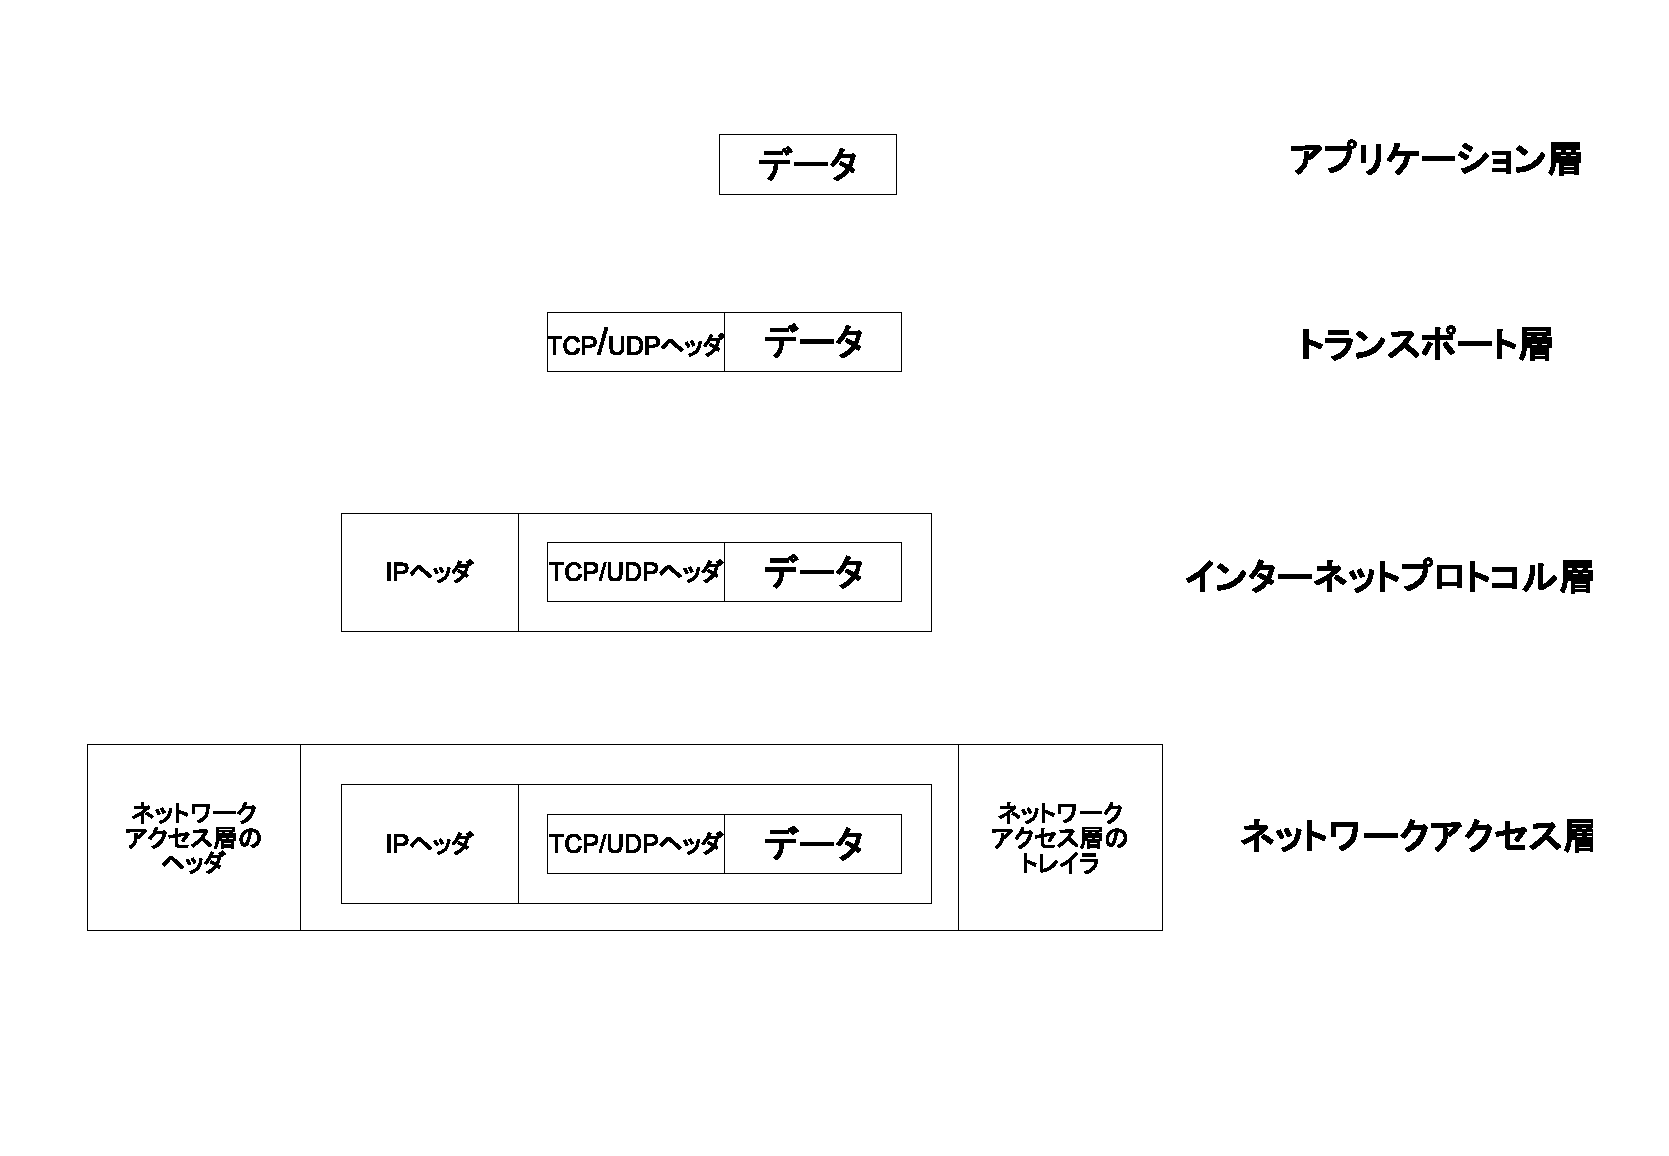
\includegraphics[width=12cm,clip]{draw/encupselation.eps}
	\caption{カプセル化}
	\label{fig:encupselation}
\end{figure}

TCP/IPのように、複数のレイヤからなるプロトコルには、カプセル化という概念がある。この概念を、アプリケーション層からどのようにデータがネットワークコミュニケーション層に送り出されるかを見てみよう。

アプリケーション層から発行されたデータは、トランスポート層で扱えるデータにしてやらないと、トランスポート層から送り出すことができない。
トランスポート層から送り出せるデータにするには、トランスポート層のデータとして必要なデータを追加する。具体的伊は、アプリケーション層のデータの先頭に、トランスポート層のヘッダを付加する。また、インターネットプロトコル層で扱えるデータのサイズに切り分けることも、トランスポート層で行う。

通信に使うための情報部分を、データの先頭にあることか羅、ヘッダ情報、あるいは単にヘッダという。ネットワークコミュニケーション層では末尾に着けることもあり、そのような付加情報をトレイラとよぶ。
また、上位レイヤーから受け取ったデータを、ペイロードと呼ぶ。

あるレイヤーが、上位のレイヤーのデータを加工して、自分のレイヤーのデータにしてから、会のレイヤーに渡すことを、カプセル化と呼ぶ。粉薬をカプセルに入れて、固形の薬という形に変えるイメージでカプセル化と呼ぶ。
このカプセル化は、アプリケーション層のデータをトランスポート層に送り出すときだけではない。トランスポート層から送り出されたデータは、インターネットプロトコル層で扱えるようにする必要がある。このときも、インターネットプロトコル層に必要なデータを付加する、カプセル化が行われる。
更に、インターネットプロトコル層からネットワークアクセス層にデータが送り出される際も、同様にカプセル化が行われる。

最終的に、アプリケーション層のデータは、トランスポート層、インターネットプロトコル層、ネットワークアクセス層という三重のカプセルに包まれて、ビット列としてネットワークに送り出されるされる。

\subsection{カプセルをはがす}
では、受信側に届いたデータはどうなるのであろうか。データを受信したネットワークコミュニケーション層は、ネットワークコミュニケーション層で通信するためのデータを外し、インターネットプロトコル層にデータを渡す。インターネットプロトコル層、トランスポート層でも同様に、自分が通信に使うデータを外して、一つ上のレイヤに残りデータを渡す。

最終的に、アプリケーション層は、送信元のアプリケーション層が発信したデータのみ受け取る。

\subsection{トンネリング}
トンネリングという言葉には、二つの似て異なる意味がある。それは、エンドツーエンドにおける、設計思想としてのトンネリングと、プロセス間通信の手段に一般名称としてのトンネリングである。

\subsubsection{設計思想としてのトンネリング}

設計思想としてのトンネリングは、カプセル化を、通信のエンドから見た視点で説明したものである。

インターネットプロトコルスイートのあるレイヤとレイヤの間の通信は、いわば同じ階層にあるレイヤの間でトンネルを通して、途中に何があるかを無視して、直接向かい合っているイメージである。そのため、同じ階層にあるあるレイヤからレイヤへの通信を、トンネリングという。これは、エンドツーエンド原則における、通信の両端のトランスポート層、アプリケーション層は、そのしたの経路が何であれ、直接通信をしているものとしてやりとりする、ということである。


\subsubsection{プロセス間通信の手段としてのトンネリング}

トンネリングにはもう一つの側面がある。同じ階層にあるレイヤからレイヤの通信は、かならずしもひとつ下のレイヤの通信を使う必要はない。例えば、ネットワークコミュニケーション層のフレームのビット列を、アプリケーションのストリームとしてして送ったと考えてみよう。
そうすれば、本来は同じネットワークでしかできないネットワークコミュニケーション層の通信が、違うネットワークに置かれた機器同士で可能となる。
当然、エンドにはそれぞれ、ネットワークアクセス層のフレームをキャプチャし、それをアプリケーションのデータとして送り出すアプリケーションを動かしておかなければならない。

また、インターネットプロトコル層のペイロードとして、IPデータグラムを載せて通信することで、インターネットプロトコルでは直接通信できない
ネットワーク間の通信が可能となる。これが、VPN(Virtual Private Network)の概念である。
\section*{}
\begin{itembox}[l]{いもうとコラム 闘士ゴーディアン}
1979年に放送された、闘士ゴーディアンというタツノコプロのロボットアニメを知っていますか、あるいは、覚えていますか。
この作品の主役ロボットは、いわば着用型のパワードスーツです。

主人公のダイゴ大滝は、プロテッサーという小型ロボットを着用します。
ユニークなのはここからで、プロテッサーは、デリンガーという一回り大きいロボットを着用します。更にデリンガーは、ガービンというもう一回り大きいロボットを着用します。

長々とゴーディアンの話をしたのは、TCP/IPにおけるカプセル化のイメージがまさにこの形だからです。アプリケーション層のデータがダイゴ大滝であるとすれば、プロテッサー、デリンガー、ガービンの着用は、各層のカプセル化に相当する、というわけです。

余談ながら、ゴーディアンは玩具先行のデザインなので、DX超合金では、関節の処理に破綻がありません。ダイゴ大滝、プロテッサー、デリンガー、ガービンと着用した状態で、ガービンの間接が稼動するという今見てもすごいおもちゃです。


\end{itembox}


\section{TCP/IPとOSI参照モデル}
ネットワークの役目を層として表すものとして、OSI参照モデル(Open Systems Interconnection Reference Model)\footnote{レイヤーが七つあることから、OSI7階層モデルと記載されることもある}、と呼ばれるモデルがある。OSI参照モデルは、TCP/IPとは全く別に、IEEEによって制定された規格である。

古いネットワークの教科書では、TCP/IPでなく、OSI参照モデルが取り上げられていることがある。かつては、研究所発祥のTCP/IPは、そのうち役目を終えて、OSI参照モデルという正しい存在に置き換えられると洋装されていた。
だが、実際には、TCP/IPは研究所のネットワークを飛び出し、世界中でネットワークを繋ぐために使われている。

OSI参照モデルは七つのレイヤを持つ。そのレイヤの名前と、対応するレイヤ番号は、表\ref{osirm}となる。

\begin{table}[hbtp] 
\begin{center} \label{osirm}
	\begin{tabular}{cl} \toprule 
		レイヤ番号 & レイヤ名 \\ \midrule
		L7 & アプリケーション層 \\
		L6 & プレゼンテーション層 \\
		L5 & セッション層 \\
		L4 & トランスポート層 \\
		L3 & ネットワーク層 \\
		L2 & データリンク層 \\
		L1 & 物理層 \\ \bottomrule
	\end{tabular}
\end{center} \caption{OSI参照モデル}
\end{table} 

TCP/IPとOSI参照モデルをにマッピングして説明することが多い。それは、機能がおおまかにマッピングできるからである。

たとえば、TCP/IPのネットワークコミュニケーション層は、OSI参照モデルでは、物理層とデータリンク層をあわせたものに相当するとされる。同様に、OSI参照モデルのネットワーク層はインターネット層、OSI参照モデルのトランスポート層はTCP/IPでもトランスポート層に相当する。また、OSI参照モデルのそこから上の層は、TCP/IPのアプリケーション層に相当する。名前は同じだが、OSI参照モデルとインターネットプロトコルスイートのアプリケーション層とが、直接対応しているわけではない。

このように、OSI参照モデルとインターネットプロトコルスイートは、一対一でマッピングすることができない。それが、大まかにマッピングできるという表現になった理由である。
また、TCP/IPのある層の機能が、OSI参照モデルでは複数の層にまたがっていたり、OSI参照モデルのある層の機能が、TCP/IPでは対応するとされている層には実装されていなかったりするという事情もある。では、そのような例を、いくつか挙げてみよう。

前述の通り、インターネットプロトコルスイートのネットワークコミュニケーション層はOSI参照モデルでは物理層とデータリンク層になる。また、OSI参照モデルのトランスポート層に対応するインターネットプロトコルスイートのトランスポート層の機能の一部は、OSI参照モデルのセッション層にも含まれている。

また、インターネットプロトコルスイートでは、回線の全二重、半二重の判別が必要であれば、ネットワークコミュニケーション層以下で実装される。だが、OSI参照モデルでは回線の全二重、半二重の判別とそれぞれに対応した通信は、セッション層で実現することになっている。

OSI参照モデルのレイヤ3であるネットワーク層では、確実な通信を行うためのコネクション型通信と、そうでない場合のコネクションレス通信の両方が規定されている。だが、TCP/IPのインターネットプロトコル層は、コネクションレス通信のプロトコルである。コネクション型のプロトコルは、その上位のトランスポート層が担当する。

OSI参照モデルでは、トランスポート層がエラー訂正の機能を持つとされている。だが、TCP/IPには、エラー訂正の機能はない。データの破損を検出する機能は存在する。だが、その場合は単にデータを破棄する。そして、確実に届かなければならないデータであれば、相手が再送することを期待する。
インターネットプロトコルスイートの通信で、エラー訂正が必要であれば、アプリケーション層が送出するデータにエラー訂正のための冗長な情報を含めておくか、ネットワークアクセス層で同様に実現するかとなる。ネットワークアクセス層でエラー訂正機能を実装する必要があるのは、たとえば、衛星通信のように、エラー訂正の情報でデータが大きくなる以上に、エラーによる再送のコストが高くなる場合に行われる。


\subsection{OSI参照モデルとネットワーク機器の機能}
現在では、OSI参照モデルは、その概念のみが残っており、OSI参照モデルをリファレンスにした実装は存在しない。
現在では、OSI参照モデルは、ネットワーク機器の機能を表すための用語として、レイヤ番号のみが使われている。この、レイヤ番号を用いた表見は、ネトワークやインフラのエンジニアが用いることが多い。

先ほど説明したように、TCP/IPとOSI参照モデルのレイヤーは一対一対応しているわけではない。だが、ネットワーク機器の機能を表現するのには、ネットワークコミュニケーション層機器ではなくL(レイヤ)2機器というような言い方をする。同様に、インターネットプロトコル層機器でなくL3機器、というように、インターネットプロトコルスイートの各層と「おおむね対応している」OSI参照モデルの層のレイヤ番号を用いる。

ネットワーク機器のスイッチングHUBは、インターネットプロトコルスイートでは、ネットワークコミュニケーション層に対応する機器である。そのため、ネットワークコミュニケーション層におおむね対応するOSIのレイヤ番号を用いて、L2スイッチ、あるいはレイヤ2スイッチと呼ぶ。SW-HUBが用いるネットワークコミュニケーション層での機能は、OSI参照モデルでは下から2層目、データリンク層に相当する機能の機器であるためだ。

唯一の例外はL1で、レイヤー1でなく、物理層と呼ばれることが多い。たとえば、ケーブルの断線は物理層ので発生した障害である。
だが、光ファイバの中の信号を、光学的に多重化するPONや、光とイーサネットのメディアコンバータなど、インターネットプロトコル層に直接サービスしない機器は、L1機器とよばれることがある。

また、TCP/IPでインターネットプロトコル層の機器であるルータは、OSI参照モデルではおおむねネットワーク層に相当するとされる。そのため、ネットワーク層のレイヤ番号3を用いて、L3機器と表現する。また、L3スイッチという機器は、見た目こそスイッチングHUBであるが、インターネットプロトコル層の機能を持っていることを意味する。

\subsection{高レイヤ機器}

ネットワーク機器には、L4機器、L5機器、L7機器と呼ばれる機器もある。
これらの機器は、L2やL3の機器と対比して、高レイヤ機器と呼ばれることがある。

\subsubsection{L4機器}

L4の機器はトランスポート層に対応する。L5の機器は、セッション層、L7の機器は、アプリケーション層である。
これらの高レイヤ機器は何を行うための機器なのだろうか。

L4の機器は、インターネットプロトコル層のIPアドレスと、レイヤ4におおむね対応するトランスポート層のポート番号を識別する。それを利用することで、通信がどのサーバのどのアプリケーションにタイして行われているかを判別する。
IPアドレスとポート番号の情報を利用して、通信を許可するかどうかを判別するファイアウォールが、代表的なL4機器である。

\subsubsection{L5機器}

L5は、TCP/IPと対比するとき、トランスポート層とアプリケーション層の中間という位置づけになる。
そのため、トランスポート層とアプリケーション層の中間でストリームを暗号化するSSL/TLSを、L5に対応づけることがある。\footnote{SSL/TLSは、アプリケーションのストリームを暗号化するという動作から、どうしてもOSI参照モデルに対応づけたいなら、L6に置くべきと考えられる。}

L5に割り当てたSSL/TLSを、SSLアクセラレータやSSL-VPNとして提供する機器が、L5機器と言われることがある。

\subsubsection{L7機器}

L7機器は、レイヤ7におおむね対応するアプリケーション層のプロトコルとその状態を判別して、通信を制御する。
たとえばWebサーバが複数ある環境で、どれかのサーバに接続するという方法で負荷を分散しつつ、特定のサーバに接続し続ける必要がある、HTTPのセッション維持を行う、ロードバランサを実現することがが可能となる。

また、アプリケーションプロトコルのデータを監査してウィルスやマルウェアのチェックを行うスクリーニング用のプロキシをL7機器と呼ぶこともある。さらに、Webサーバへのアクセスをスクリーニングするソフトウェアとsちえ実装され宇WAF(Web Application Firewall)も、ネットワークから見れば、L7相当となる。

\subsection{OSI参照モデルのL8、L9、L10}

パイソンズのスケッチ、スペイン宗教裁判\footnote{Nobody expects the Spanish Inquisition!}ではないのだが、七階層あるOSI参照モデルには、レイヤ8からレイヤ10までの3層が存在する。
スペイン宗教裁判では、罪が三つしかないはずなのに、、異端審問官が四つ数え上げる、というのが笑うところだが、OSI参照モデルは、七層のはずが実際には十層のレイヤーで構成されている。
その構成は、L8が経済層、L9が政治層、L10が宗教層となるとするもの、L8がユーザ層、L9が経済層、L10が宗教層とするものなど、諸説ある。

ここまで説目下が、L8から上は、OSIの公式の規格ではなくジョークの類である。

ネットワークの問題は、往々にして、ネットワークの外で、技術的では内理由によって発生する。つまり、事件はデータセンタで起きても障害は会議室で起こるのだ。それは経済的事情で機器やそのサポートが買えない、社内政治の事情でベンダや代理店が変更される、上司がクラウドを使わなければ安全、という宗教的な進行に捕らわれている、など、現場ではどうにもならない理由で発生する障害を皮肉ったものだ。

つまり、L8以上の問題とは、技術的に解決できるはずのことが解決できない状況である。そして、本書で取り扱い範囲を超えるため、詳細は割愛する。

